The starting point in the remainder of this work will be the set of events belonging to a particular uncertain process instance.
From now on, we always assume we are given an uncertain log $L \subseteq \mathcal{E}$.
For every case $c \in \mathcal{U}_C^L$ and its corresponding event set $E_c$, we aim to estimate the probability of each possible activity trace corresponding to it.
For ease of notation, we omit the subscript $c$ when the case is clear from the context.

\section{Splitting of Uncertain Traces}
Now we show a naive method to compute the topological sortings of a directed acyclic graph through the \textsc{TopologicalSortings} algorithm (Algorithm \ref{alg:topo sortings}). 
Note that when the input graph is the follows graph of some event set $E$, according to Theorem \ref{theorem: topological sortings}, the topological sortings are equivalent to the correct evaluation orders on $(E,\prec_{\mathcal{E}})$.

\begin{algorithm}[h!]
	\caption{\textsc{TopologicalSortings($G$)}}
	\label{alg:topo sortings}
	\SetKwInOut{Input}{Input~}
	\SetKwInOut{Output}{Output~}
	\Input{~A directed graph $G=(V,A)$.}
	\Output{~Set $\mathcal{O}$ of topological sortings of $G$.}
	
	$\mathcal{S} \gets \mathcal{S}_V$ \tcp*{Set of all permutations over set $V$} \label{2: 1}
	
	\If{$|A| = 0$}{ \label{2: 2}
		\Return $\mathcal{S}$ \tcp*{All permutations are valid if $G$ has no arcs} \label{2: 3}} 
		
	$\mathcal{O} \gets \{ ~ \}$	\tcp*{Initialize set of valid permutations}
	
	\For{$s \in \mathcal{S}$}{ \label{2: 5}
		$previous \gets \{ ~ \}$ \tcp*{Events from $previous$ shouldn't appear \\ \label{2: 6}
		 later in $s$}
		$i \gets 1$
		
		\While{$i \leq |V|$}{ \label{2: 8}
			$current = s[i]$\\  \label{2: 9}
			\If{$i = |V|$}{ \label{2: 10}
				\If{$current \not \in previous$}{
					$\mathcal{O} \gets \mathcal{O} \cup {s}$ \label{2: 12}
					}
				}
			\Else{
				$incoming \gets \delta^{-}(s[i])$ \\ 
				\If{$(i=1 \wedge |incoming|>0) \vee current \in previous $ \label{2: 15} } 
				{
					\textbf{break} \tcp*{$s$ invalid, continue with next permutation} \label{2: 16}
					}
				$previous \gets previous \cup incoming$ \label{2: 17}	
				}
			}
		}
	\Return $\mathcal{O}$
	

\end{algorithm}

The algorithm goes through all permutations over the vertex set (line \ref{2: 5}) and adds the valid ones (the topological sortings) to set $\mathcal{O}$.
For a directed graph $G=(V,A)$ where $A$ is the set of arcs and a particular vertex $v \in V$: 
$\delta^-(v)=\{u \in V \mid (u,v) \in A\}$ is the set of incoming neighbours of vertex $v$.
Note that if the current permutation is indeed a valid one, when encountering any vertex $v$ on position $i$, all vertices from $\delta^-(v)$ should have appeared previously in the permutation.
Otherwise, the permutation is not a topological sorting (Definition \ref{def: topological sorting} and Lemma \ref{lemma: edge path}).
For this reason, set $previous$ is created for each permutation (line \ref{2: 6}) to contain all the vertices that should not appear later in the permutation.
We go through all vertices in their order of appearance in each permutation (lines \ref{2: 8}-\ref{2: 9}), and add their incoming neighbors to set $previous$ in line \ref{2: 17}.
If we later encounter some vertex from $previous$ in the current permutation, we discard the permutation as invalid and break (lines \ref{2: 15}-\ref{2: 16}).
Another reason to discard a permutation as invalid is if the current vertex is the first one in the current permutation and it already has incoming neighbors, meaning vertices which should not appear after it (lines \ref{2: 15}-\ref{2: 16}).
We add the current permutation to the set of topological sortings in lines \ref{2: 10}-\ref{2: 12} if we make it to its last element without discarding it.

Note that it is the set of arcs in the input graph that poses constraints for the order of appearance of the vertices. 
If there are no arcs, then every permutation of the vertex set is valid (lines \ref{2: 2}-\ref{2: 3}). 

Computing $\mathcal{O}_G$ requires going through all permutations in $\mathcal{S}_V$ (a total number of $|V|!$ ) in order to obtain the ones which are a topological sorting.
When $V$ corresponds to a rather big event set, this might be problematic.
However, there might be many traces where despite uncertainty in timestamps, one can still partition the set of events of a case into smaller subsets which certainly happened sequentially. 
Think for example of processes with rather long traces where overlapping timestamps appear only in local parts of the process.
When the event set is timely partitioned, the task of computing $\mathcal{O}_G$ is reduced to computing the topological sortings (and this way the correct evaluation orders) on the smaller subsets.
Depending on how well the uncertain trace can be fragmentized, this may help making the computation much more efficient.
Next we explain how to obtain  these subsets.
%
%
% 

\begin{definition}[Comparability Graph]\label{def: comparability graph}
Let $E$ be the event set belonging to a process instance from some uncertain event log $L$.
The \emph{comparability graph} $\mathcal{C}omp(E)=(V_{\mathcal{C}omp},E_{\mathcal{C}omp})$ of event set $E$ is constructed as follows:
$V_{\mathcal{C}omp} = E$ and
$E_{\mathcal{C}omp} = \{ \{u,v\} \mid u \prec_{\mathcal{E}} v \vee v \prec_{\mathcal{E}} u\}$.
\end{definition}

\begin{proposition} \label{prop: comp = undirected}
Given an event set $E$, the comparability graph $\mathcal{C}omp(E)=(V_{\mathcal{C}omp},E_{\mathcal{C}omp})$ is the undirected variant of the follows graph $\mathcal{F}(E)=(V_{\mathcal{F}},E_{\mathcal{F}})$.
\end{proposition}

\begin{proof}
Let $\mathcal{F}(E)^U=(V_{\mathcal{F}}^U,E_{\mathcal{F}}^U)$ be the undirected variant of $\mathcal{F}(E)$ as defined in \ref{def: undirected variant}.
It holds that $V_{\mathcal{C}omp} = E = V_{\mathcal{F}} = V_{\mathcal{F}}^U$ by Definitions \ref{def: comparability graph}, \ref{def: follows graph} and \ref{def: undirected variant} respectively.
Additionally, it holds that $\{u,v\} \in E_{\mathcal{C}omp} 
\overset{Def.\ref{def: comparability graph}}{\Longleftrightarrow} 
u \prec_{\mathcal{E}} v \vee v \prec_{\mathcal{E}} u 
\overset{Def. \prec_{\mathcal{E}}}{\Longleftrightarrow}
(u \prec_{\mathcal{E}} v \vee v \prec_{\mathcal{E}} u) \wedge u \neq v
\overset{Def.\ref{def: follows graph}}{\Longleftrightarrow}
((u,v) \in E_{\mathcal{F}} \vee (v,u) \in E_{\mathcal{F}}) \wedge u \neq v
\overset{Def.\ref{def: undirected variant}}{\Longleftrightarrow}
\{u,v\} \in E_{\mathcal{F}}^U$.
%\qed
\end{proof}
 
The comparability graph is undirected and it contains an edge between a pair of events $e,e' \in E$ if and only if their time intervals are comparable, that is, there is no overlapping of their possible timestamps.
By ignoring the direction of the arcs in the follows graph, the comparability graph focuses on comparability instead of the predecessor/successor relationship.


\begin{definition}[Interval Graph]\label{def: interval graph}
Let $E$ be the event set belonging to a process instance from some uncertain event log $L$.
The \emph{interval graph} of event set $E$ is the graph $\mathcal{I}(E)=(V_{\mathcal{I}},E_{\mathcal{I}})$ where
$V_{\mathcal{I}} = E$ and 
$E_{\mathcal{I}} = \{ \{u,v\} \mid t_{min}(u) \leq t_{max}(v) \wedge t_{min}(v) \leq t_{max}(u)\}$.
\end{definition}
Note that in the interval graph, two events are connected by an edge if and only if they have overlapping timestamps.
%\begin{proposition}
%Let $\mathcal{I}(E)=(V_{\mathcal{I}},E_{\mathcal{I}})$ be the interval graph of some event set $E$.
%Given $u,v \in V_{\mathcal{I}}$, it holds that $\{u,v\} \in E_{\mathcal{I}}$ if and only if $u$ and $v$ are not comparable w.r.t. $\prec_{\mathcal{E}}$.
%\end{proposition}

%\begin{proof}
%Let $u$ and $v$ be two events which have overlapping timestamps, that is, they are not comparable w.r.t $\prec_{\mathcal{E}}$.
%It holds that $u,v \in E$ not comparable w.r.t. $\prec_{\mathcal{E}} \Leftrightarrow
%u \not \prec_{\mathcal{E}} v \wedge v \not \prec_{\mathcal{E}} u
%\Leftrightarrow
%t_{max}(u) \not < t_{min}(v) \wedge t_{max}(v) \not < t_{min}(u)
%\Leftrightarrow
%t_{max}(u) \geq t_{min}(v) \wedge t_{max}(v) \geq t_{min}(u)
%\Leftrightarrow
%\{u,v\} \in E_{\mathcal{I}}$.
%\qed
%\end{proof}
%


\begin{proposition}\label{prop: interval = complement}
Given an event set $E$, the interval graph $\mathcal{I}(E)=(V_{\mathcal{I}},E_{\mathcal{I}})$ is the complement of the comparability graph $\mathcal{C}omp(E)=(V_{\mathcal{C}omp},E_{\mathcal{C}omp})$.
\end{proposition}

\begin{proof}
Let $\overline{\mathcal{C}}=\overline{\mathcal{C}omp(E)}=(V_{\overline{\mathcal{C}}}, E_{\overline{\mathcal{C}}})$ be the complement of the comparability graph $\mathcal{C}omp(E)=(V_{\mathcal{C}omp},E_{\mathcal{C}omp})$ of event set $E$.
It holds that $V_{\mathcal{I}}=E=V_{\mathcal{C}omp}=V_{\overline{\mathcal{C}}}$ by Definitions \ref{def: interval graph}, \ref{def: comparability graph} and \ref{def: complement graph} respectively.
Additionally, it holds that 
$ \{u,v\} \in E_{\mathcal{I}}
\overset{Def. \ref{def: interval graph}}{\Longleftrightarrow}
t_{min}(u) \leq t_{max}(v) \wedge t_{min}(v) \leq t_{max}(u)
\overset{}{\Longleftrightarrow}
\neg \big( t_{min}(u) > t_{max}(v) \vee t_{min}(v) > t_{max}(u) \big)
\overset{Def. \prec_{\mathcal{E}}}{\Longleftrightarrow}
\neg \big( v \prec_{\mathcal{E}} u \vee u \prec_{\mathcal{E}} v \big)
\overset{Def. \ref{def: comparability graph}}{\Longleftrightarrow}
\{u,v\} \not \in E_{\mathcal{C}omp}
\overset{Def. \ref{def: complement graph}}{\Longleftrightarrow}
\{u,v\} \in E_{\overline{\mathcal{C}}}
$.
%\qed
\end{proof}


\begin{theorem}\label{theorem: partitioning}
Let $\mathcal{I}(E)=(V_{\mathcal{I}},E_{\mathcal{I}})$ be the interval graph of some event set $E$.
The connected components of $\mathcal{I}(E)$ partition set $E$ into subsets of minimal size such that any two events from different subsets can be ordered in time.
\end{theorem}


\begin{proof}
\leavevmode \\ 
(1) \textit{Any two events from different components of the interval graph appear in the $\prec_{\mathcal{E}}$ relation.}\\
Suppose that $C_1, C_2 \subseteq V$ are two connected components of $\mathcal{I}(G)$ and let $e_1 \in C_1, e_2 \in C_2$ be two arbitrary vertices (representing events $e_1$ and $e_2$) from these components.
We know that $\{e_1,e_2\} \not \in E_{\mathcal{I}}$.
Since the interval graph is the complement graph of $\mathcal{C}omp(E)$ (Prop. \ref{prop: interval = complement}), then $\{e_1,e_2\} \in E_{\mathcal{C}omp}$.
By definition of the comparability graph, either $e_1 \prec_{\mathcal{E}} e_2$ or $e_2 \prec_{\mathcal{E}} e_1$ must hold.
W.l.o.g assume that $e_1 \prec_{\mathcal{E}} e_2$.
Then $t_{max}(e_1) < t_{min}(e_2)$ and thus events $e_1$ and $e_2$ can be ordered. \\ \\
(2) \textit{There is no finer partition on the event set that satisfies (1) than the one induced by the connected components of the interval graph.}\\
Let $\mathcal{I}(E)$ be the interval graph of $E$  and let $V= C_1 \cup ... \cup C_n$ be its partition into connected components for which (1) holds.
Assume there is some component $C$ from $\{C_1,...,C_n\}$ which can be further partitioned into two non-empty subsets $C=C' \cup C''$ so that claim (1) still holds.
Let $e' \in C', e'' \in C''$ be two arbitrary vertices from $C'$ and $C''$.
Since $e',e'' \in C$, it holds that $\{e',e''\} \in E_{\mathcal{I}}$. 
Because the interval graph is the complement of the comparability graph $\mathcal{C}omp(E)$, then $\{e',e''\} \not \in E_{\mathcal{C}omp}$.
This means that both $e' \not \prec_{\mathcal{E}} e''$ and $e'' \not \prec_{\mathcal{E}} e'$ hold.
That is the case when both $t_{max}(e') \not < t_{min}(e'')$ and 
$t_{max}(e'') \not < t_{min}(e')$ hold.
This contradicts the assumption that $C'$ and $C''$ satisfy (1). $\lightning$
%\qed
\end{proof}

\begin{proposition}\label{prop: clique}
Let $\mathcal{I}(E)=(V_{\mathcal{I}},E_{\mathcal{I}})$ be the integral graph of some event set $E$ and let $C \subseteq V_{\mathcal{I}}$ be some connected component of $\mathcal{I}(E)$.
If $C$ is a clique then every permutation $s \in \mathcal{S}_C$ is a correct evaluation order on $(C,\prec_{\mathcal{E}})$.
\end{proposition}

\begin{proof} 
Let $C=\{e_1,...,e_{|C|}\}$ be a connected component of $\mathcal{I}(E)$ which is a clique.
Then $\forall i,j \in \{1,...,|C|\}$ s.t. $i\neq j$, the pair $e_i, e_j$ is connected through an edge in $\mathcal{I}(E)$.
Since the interval graph $\mathcal{I}(E)$ is the complement of the comparability graph $\mathcal{C}omp(E)$, it holds from Prop. \ref{prop: interval = complement} that for every such pair of vertices, there is no edge between them in $\mathcal{C}omp(E)$.
This implies that $\forall i,j \in \{1,...,|C|\}$ s.t. $i \neq j$, neither $e_i \prec_{\mathcal{E}} e_j$ nor $e_j \prec_{\mathcal{E}} e_i$ hold.
This way, for every permutation $s \in \mathcal{S}_C$, the condition
$\forall ~ 1 \leq i < j \leq |s|: ~ s[j] \not \prec_{\mathcal{E}} s[i]$ is always satisfied.
Therefore, every $s \in \mathcal{S}_C$ is a correct evaluation order on $(C, \prec_{\mathcal{E}})$. \\ 
%\qed 
\end{proof}

The claim in Proposition \ref{prop: clique} is not surprising since it is equivalent to saying that all permutations of an event set are valid if their corresponding follows graph has no arcs.


%$(\Leftarrow)$
%Let $C=\{e^C_1,...,e^C_{|C|}\}$ be a set of events for which every permutation $s \in \mathcal{S}_C$ is a correct evaluation order on $(C,\prec_{\mathcal{E}})$.
%Then from Definition \ref{eval} follows that there are no $i,j \in \{1,...,|C|\}, i\neq j$ such that $s[i] \prec_{\mathcal{E}} s[j]$.
%Otherwise, every permutation where $s[j]$ appears before $s[i]$ would not be a correct evaluation order on $(C,\prec_{\mathcal{E}})$.
%This is equivalent to the claim: For every pair $i,j \in \{1,...,|C|\}, i\neq j$ it holds that neither $e^C_i \prec_{\mathcal{E}} e^C_j$ nor $e^C_j \prec_{\mathcal{E}} e^C_i$ hold.
%From Definition \ref{comp graph} of the comparability graph follows that $(e^C_i,e^C_j) \not \in E_{\mathcal{C}}$


\begin{proposition}\label{prop: component size}
Let $E$ be some event set and let $\mathcal{F}(E)$ be its corresponding follows graph.
If $\mathcal{F}(E)$ has more than one connected component, then only one of these components has size greater than 1.
\end{proposition}


\begin{proof}
%Let $E$ be some event set and let $\mathcal{F}(E)$ be its corresponding follows graph.
Assume there are two connected components $C', C''$ in $\mathcal{F}(E)$ which both have size greater than 1.
Note that we can always find two events from each component: $e_1, e_2 \in C'$ and $e_3, e_4 \in C''$,
such that both arcs $(e_1,e_2)$ and $(e_3,e_4)$ exist in $\mathcal{F}(E)$.
From the definition of the follows graph, we know that the following hold: 
$t_{max}(e_1) < t_{min}(e_2)$ and $t_{max}(e_3) < t_{min}(e_4)$.
Also, since the pairs lie in different connected components of $\mathcal{F}(E)$, there is no arc $(u,v)$ in $\mathcal{F}(E)$ such that $u \in C'$ and $v \in C''$ or vice-versa.
Since there is no arc between $e_3$ and $e_2$, it holds that $t_{min}(e_2) \leq t_{max}(e_3)$ (because $t_{max}(e_3) \not < t_{min}(e_2))$. 
From this follows:
$t_{max}(e_1) < t_{min}(e_2) \leq t_{max}(e_3) < t_{min}(e_4)$.
But this implies that $t_{max}(e_1) < t_{min}(e_4)$ so there must be an arc between $e_1$ and $e_4$.
$\lightning$
%\qed
\end{proof}
%\textcolor{red}{Note:}
Equivalently, the claim in Proposition \ref{prop: component size} can be proved by showing that every interval graph is chordal (it has no cycle of length $\geq$ 4).
%\begin{proposition}
%Let $E$ be some event set and let $\mathcal{F}(E)$ and $\mathcal{I}(E)$ be its corresponding follows and interval graph respectively.
%Let $C_1,...,C_n$ be the connected components of the interval graph $\mathcal{I}(E)$.
%For all $i=1,..,n$ it holds that $\mathcal{F}(E)[C_i]$ has at most one connected component of size greater than 1.
%\end{proposition}
%\begin{proof}
%Follows directly from Proposition \ref{comp size}.
%\end{proof}
Propositions \ref{prop: clique} and \ref{prop: component size} contain two claims which we will exploit when constructing the set of correct evaluation orders in the next section.
Proposition \ref{prop: clique} says that if a connected component of the interval graph is a clique, then all permutations of its vertices induce topological sortings and thus also correct evaluation orders.
If the subgraph is not a clique, then we have to look at the corresponding follows graph in order to obtain the topological sortings.
According to Proposition \ref{prop: component size}, in this subgraph there is at most one connected component with more than one node and thus a non-trivial set of topological sortings. 
From here on, one could repeat the same reasoning for the subgraphs of the follows graph: using their interval graphs to split  them and then repeat the procedure until we arrive at trivial components of size one.
One would then have to merge their corresponding permutations step by step into full sequences.
The way the smaller subsequences should be merged depends on whether the graph components they were part of during the split belonged to the follows graph or the interval graph.
This is the idea behind the method that we introduce in the next section.
%
%
%
%
\section{Computing Event Trace Realizations: A New Approach}
Algorithm \ref{alg:valid permutations} computes the set of event trace realizations of a given event set $E$ in a non-naive way by exploiting the claims from Theorem \ref{theorem: partitioning}, Propositions \ref{prop: clique} and \ref{prop: component size}.
It relies on the following two arguments:
\begin{itemize}
\item Let $G$ be some directed acyclic graph with connected components $C_1,..,C_n$ where w.l.o.g. $C_1$ is the (only) big component.
Let $\mathcal{S}_1$ be the set of topological sortings of $G[C_1]$.
Then each permutation $s \in \mathcal{S}_{V(G)}$ is a topological sorting in $G$ if and only if there exists $s_1 \in \mathcal{S}_1$ such that the elements of $s_1$ appear in $s$ in the same order: $s \downharpoonright_{C_1} = s_1$ ($s$ projected onto set $C_1$).
%\textcolor{red}{This is a bit complicated in the algorithm, corresponding part in the swappingAlg must be changed. It has to be done because it is still better than going through all permutations. Otherwise one could remove the whole recursive method and just do naive topological sorting on the first-level connected components of the interval graph}.
\item Given some follows graph $\mathcal{F}$ and its corresponding interval graph $\mathcal{I}$ which has $m$ connected components, one can timely order the components into $\langle C_1,...,C_m \rangle$ such that $\forall ~ 1 \leq i<j \leq m: ~ e_i \prec_{\mathcal{E}} e_j$ for every pair $e_i \in C_i$ and $e_j \in C_j$.
This follows from Theorem \ref{theorem: partitioning}.
Moreover, the topological sortings of $\mathcal{F}$ are the sequences $\langle s^1,...,s^m \rangle$ such that $s^i$ is a topological sorting of $\mathcal{F}[C_i]$ for all $i \in \{1,...,m\}$.
\end{itemize}
These two points constitute the idea behind our new method for computing the event trace realizations.
%On one hand, we use Algorithm \ref{alg: FollowsGraph Splitting} to handle each connected component of the follows graph separately.
%The valid permutations of these components are merged together using Algorithm \ref{alg:combine with}.
%The name \textsc{CombineWithSwapping} of Algorithm \ref{alg:combine with} indicates that any order of the sequences emerging from different follows graph components is valid. 
%The \textsc{Interweave} method used in Algorithm \ref{alg:combine with} exploits the knowledge that only one component might be of size greater than 1 to compute the merges more efficiently.
%For each component of the interval graph on the other hand, Algorithm \ref{alg: IntervalGraph Splitting} handles the connected components of the interval graph and detects their ordering.
%Their valid sequences are then merged together according to this order using Algorithm \ref{alg:combine without}.
%The name \textsc{CombineWithoutSwapping} of Algorithm \ref{alg:combine without} indicates that the components' order in the interval graph is fixed and no swapping takes place.
%
%Algorithms \ref{alg: FollowsGraph Splitting} and \ref{alg: IntervalGraph Splitting} call each-other interchangeably to efficiently make use of the graph structure to prune all invalid permutations of the vertices.
%The recursion breaks when the graph for which the valid permutations have to be computed has a single node.
%The recursion might be stopped earlier if in the \textsc{IntervalGraphSplitting} method it is noticed that the interval graph of a given connected follows graph still has no more than one single component.
%Here the algorithm relies again on the naive way using the \textsc{TopologicalSortings} method to obtain the valid permutations on that particular subgraph.
%In the end, the output of Algorithm \ref{alg:valid permutations} is a set containing all valid permutations on the input event set.
%
%
%
%
%
%
%
%
%
%
%
%
\begin{algorithm}[h!]
	\caption{\textsc{CombineWithSwapping}($\{P_1,...,P_k \}$)}
	\label{alg:combine with}
	\SetKwInOut{Input}{Input~}
	\SetKwInOut{Output}{Output~}
	\Input{~A set of sets $P_i$ each containing sequences.}
	\Output{~Set of (full sequences) where each is a combination of sequences from the sets $P_i$ in any possible order.}	
	
	\If{$k=1$}{
		\Return $P$ \tcp*{Nothing to merge when there is only one set}
		} 
	\If{$|P_i[1]| = 1 ~ \forall 1 \leq i \leq k$}{
		\Return $S_{\{s_1,...,s_k\}}$ \tcp*{Here all $P_i$-s are singleton sets, \\ so all permutations are valid.}}
		
		
	$FullSequences \gets \{ ~ \}$	
	
	$orderedSets \gets list(P_1,...,P_k)$ \tcp*{create some arbitrary ordering}
	
	$b \gets BigComponent(P_1,...,P_k)$ \tcp*{identifying the index of the \\ (single) set with non-trivial sequences}
	
	$swappings = \mathcal{S}_{\{1,...,k\} \setminus \{b\}}$ \tcp*{all possible swappings of singleton sets}
	
	$singletonPermutations \gets \{ ~ \}$
	
	\For{$swap \in swappings$}{
		$combinedSingletons \gets \bigotimes_{j=swap[1]}^{swap[|swap|]} P_j $	
		
		\For{$s \in combinedSingletons$}{
			$singletonPermutations \gets singletonPermutations \cup \{\widehat{s}\}$ \tcp*{All \\ permutations without the big component}
			}	
		}
	$FullSequences \gets \{~\}$ \\
	
	%\textcolor{blue}{	
	\For{$s_b \in P_b$}{ \label{3: 15}
		\For{$s \in singletonPermutations$}{
			$interweavings \gets $ \textsc{Interweave}($s_b,s$) \\
			$FullSequences \gets FullSequences \cup interweavings$
			} \label{3: 18}
		}
	%}
	\Return $FullSequences$
\end{algorithm}
%\caption{Given sets $P_1,...,P_k$ where each one contains sequences, \emph{combining} them means obtaining the (flattened) full sequences from their cartesian product, while \emph{swapping} means that all orderings of sets in the cartesian product are possible.}
%
%
%
%
%
%
%
%
%
%
%
%
\begin{algorithm}[h!]
	\caption{\textsc{Interweave}($s_b,s$)}
	\label{alg:place}
	\SetKwInOut{Input}{Input~}
	\SetKwInOut{Output}{Output~}
	\Input{~Two sequences $s_b$ and $s$ where $s_b$ comes from the big component and $s$ is a permutation of singleton sequences.}
	\Output{~A list of full sequences interweaving elements from $s_b$ and $s$ without changing the ordering.}	

	\If{$s_b=\langle ~ \rangle$ \tcp*{stop when all elements from $s_b$ were picked}}{
		\Return ${s}$}
		
	$interweavings \gets \{ ~ \} $ \\
	$event \gets s_b[1]$ \tcp*{Start with first element of $s_b$}
	
	\For{$pos \in \{0,...,|s|\}$}{
		$s_{new} \gets s$ \tcp*{create a copy of sequence $s$}
		$s_{new}.insert(pos,event)$ \tcp*{Insert event to $s$ at position $pos$} 
		$interweavings \gets interweavings \cup \{
		 \textsc{Interweave}(s_b[2:],s_{new}, pos+1) \} $  %\tcp*{insert the rest of $s_b$ }
		}
	\Return $interweavings$
		
\end{algorithm}
%
%
%
%
%
%
%
%
%
%
%
%
\begin{algorithm}[h!]
	\caption{\textsc{CombineWithoutSwapping}($\langle P_1,...,P_k \rangle$)}
	\label{alg:combine without}
	\SetKwInOut{Input}{Input~}
	\SetKwInOut{Output}{Output~}
	\Input{~A list of sets $P_i$, each containing sequences.}
	\Output{~Set of (full) sequences where each comes from the cartesian product of the $P_i$-s.}
	
	\If{$k=1$}{
		\Return $P$ \tcp*{Nothing to merge when there is only one set}
		}
		
	$FullSequences \gets \{ ~ \}$	
	
	$combinedSequences \gets \bigotimes_{i=1}^k P_i$ \tcp*{cartesian product of sets} \label{5: 4}
	
	\For{$s \in combinedSequences$}{
		$FullSequences \gets FullSequences \cup \{\widehat{s}\}$ 
		\tcp*{flatten list $s$} \label{5: 6}
		}		
	\Return $FullSequences$
\end{algorithm}
%
%
%
%
%
%
%
%
%
%
%
%
\begin{algorithm}[h!]
	\caption{\textsc{FollowsGraphSplitting($\mathcal{F},\mathcal{I},V$)}}
	\label{alg: FollowsGraph Splitting}
	\SetKwInOut{Input}{Input~}
	\SetKwInOut{Output}{Output~}
	\Input{~A directed acyclic graph $\mathcal{F}$ and its corresponding interval graph $\mathcal{I}$, $V$ a subset of their vertex set.}
	\Output{~Set $\mathcal{O}$ of topological sortings of $\mathcal{F}[V]$.}
		
	
	\If{$V=\{v\}$}{ \label{6: 1}
		\Return $\{ \{ \langle v \rangle \} \}$ \tcp*{If $V$ has only one vertex, return \\ single set with trivial topo. sorting}
		}	\label{6: 2}
	$G \gets \mathcal{F}[V]$\\ \label{6: 3}
	$components \gets CC(G)$ \tcp*{Compute connected components of $G$} \label{6: 4}
	
	%$n_c \gets |components|$
	
	$P_{sets} \gets \{ ~ \}$
	
	\For{$C \in components$}{ \label{6: 6}
		$P_i \gets \textsc{IntervalGraphSplitting}(\mathcal{F},\mathcal{I},C)$		\label{6: 7}
		
		$P_{sets} \gets P_{sets} \cup \{\{P_i\}\}$
		}	
	$\mathcal{O} \gets \textsc{CombineWithSwapping}(P_{sets})$ \label{6: 9}
	
	
	\Return $\mathcal{O}$
\end{algorithm}
%
%
%
%
%
%
%
%
%
%
\begin{algorithm}[h!]
	\caption{\textsc{IntervalGraphSplitting($\mathcal{F},\mathcal{I},V$)}}
	\label{alg: IntervalGraph Splitting}
	\SetKwInOut{Input}{Input~}
	\SetKwInOut{Output}{Output~}
	\Input{~A directed acyclic graph $\mathcal{F}$ and its corresponding interval graph $\mathcal{I}$, $V$ a subset of their vertex set.}
	\Output{~Set $\mathcal{O}$ of topological sortings of $\mathcal{F}[V]$.}
	
	
	\If{$V=\{ v\}$}{ \label{7: 1}
		\Return $\{\{ \langle v \rangle \}\}$ \tcp*{If $V$ has only one vertex, return \\ trivial topo. sorting} \label{7: 2}
		}
	
	$G \gets \mathcal{I}[V]$\\	\label{7: 3}
	$components \gets CC(G)$ \tcp*{Compute connected components of $G$} \label{7: 4}
	
	 \If{$|components| = 1$}{ \label{7: 5}
		$\mathcal{O} \gets \textsc{TopologicalSortings}(\mathcal{F}[V])$ \tcp*{If graph cannot be splitted \\ further, use naive method.} \label{7: 6}
		\Return $\mathcal{O}$	
	 	}
	 	
	$C_{list} \gets \langle ~ \rangle$ \label{7: 8}
	
	\For{$C \in components$}{
		$start \gets min\{t_{min}(e) \mid e \in C\}$
		}
		
		$C_{list} \gets C_{list} \oplus (start,C)$
	
	$\textsc{Sort}(C_{list})$ \tcp*{Sort components on their minimal timestamps} \label{7: 12}
	
	$P_{list} \gets \langle ~ \rangle$
	
	\For{$C \in C_{list}$}{ \label{7: 14}
	
		$P_i \gets\textsc{FollowsGraphSplitting}(\mathcal{F},\mathcal{I},C)$ \label{7: 15}
		
		$P_{list} \gets P_{list} \oplus P_i$		
		}
	
	$\mathcal{O} \gets \textsc{CombineWithoutSwapping}(P_{list})$ \label{7: 17}
	
	\Return $\mathcal{O}$
\end{algorithm}
%
%
%
%
%
%
%
%
%
%
\begin{algorithm}[h!]
	\caption{\textsc{ValidPermutations($E$)}}
	\label{alg:valid permutations}
	\SetKwInOut{Input}{Input~}
	\SetKwInOut{Output}{Output~}
	\Input{~An event set $E$.}
	\Output{~Set $\mathcal{R}_e(E)$ of correct evaluation orders on $(E,\prec_{\mathcal{E}})$.}

	$\mathcal{F} \gets \textsc{FollowsGraph}(E)$ \label{8: 1}
	
	$\mathcal{C}omp \gets \mathcal{F}^U$ \tcp*{Build undirected variant of $\mathcal{F}$.} \label{8: 2}
	
	$\mathcal{I} \gets \overline{\mathcal{C}omp}$ \tcp*{Build complement graph of $\mathcal{C}omp$.} \label{8: 3}
	
	$\mathcal{R}_e \gets \textsc{FollowsGraphSplitting}(\mathcal{F},\mathcal{I},V_{\mathcal{F}})$ \label{8: 4}
	
	\Return $\mathcal{R}_e$
\end{algorithm}
%
%
%
%
%
%\newpage
We first construct the follows and interval graph of the given event set in lines \ref{8: 1}-\ref{8: 3} of Algorithm \ref{alg:valid permutations}.
Then the \textsc{FollowsGraphSplitting} method is called on the follows- and interval graph with the original vertex set in line \ref{8: 4}.
The \textsc{FollowsGraphSplitting} method in Algorithm \ref{alg: FollowsGraph Splitting} handles subgraphs of the follows graph induced by the input vertex set (line \ref{8: 3}).
If the graph has a single node, the trivial permutation is returned for that subgraph (lines \ref{6: 1}-\ref{6: 2}).
Otherwise the connected components are detected (line \ref{6: 4}), and for each of those components the interval graph trick is used by calling the \textsc{IntervalGraphSplitting} method in Algorithm  \ref{alg: IntervalGraph Splitting} (lines \ref{6: 6}-\ref{6: 7}).
The valid partial permutations yielded by Algorithm \ref{alg: IntervalGraph Splitting} for each of those components are then merged back together using the \textsc{CombineWithSwapping} method (line \ref{6: 9}).
This indicates that valid permutations of different components originating from the follows graph can be combined together in any order, as long as the ordering within the component is preserved.
From Proposition \ref{prop: component size} we know that there is at most one component of size greater than 1.
Whenever that is the case, the \textsc{CombineWithSwapping} method in Algorithm \ref{alg:combine with} calls the \textsc{Interweave} function (lines \ref{3: 15}-\ref{3: 18}), which constructs all valid mergings of the singleton components with the big component.

As we mentioned, the \textsc{IntervalGraphSplitting} method in Algorithm \ref{alg: IntervalGraph Splitting} is applied on a connected component of the follows graph and handles the subgraph of the interval graph induced by the input vertex set. 
In the end it yields the valid permutations on the input vertex set of that component.
To do this, it first checks whether the input is a single vertex in line \ref{7: 1}.
If that is the case, then the trivial permutation is returned in line \ref{7: 2}.
Otherwise, the subgraph of the interval graph induced by the input vertex set is computed in line \ref{7: 3}.
The set of connected components in the subgraph of the interval graph is computed (line \ref{7: 4}) and their order is detected (lines \ref{7: 8}-\ref{7: 12}).
Each of those components represents a smaller instance of the original input, that is, smaller vertex sets for which the valid orderings have to be computed according to the arcs connecting them in the original follows graph.
At this point the next recursion round starts, where the \textsc{FollowsGraphSplitting} method is called on each component of the interval graph (lines \ref{7: 14}-\ref{7: 15}).
Since those components have a fixed ordering which was computed before, to merge them back together the \textsc{CombineWithoutSwapping} method from Algorithm \ref{alg:combine without} is used (line \ref{7: 17}).
As the name indicates, the partial permutations of the components originating from an interval graph subgraph are combined with a fixed order.
This is easily done by obtaining the cartesian product of the sets containing the valid sequences of each component (lines \ref{5: 4}-\ref{5: 6} of Algorithm \ref{alg:combine without}).
It could also happen that the corresponding interval graph of the follows graph induced by the input vertex set in the \textsc{IntervalGrapSplitting} method does not further split the vertex set into smaller sets.
Continuing the recursion with the \textsc{FollowsGraphSplitting} method here would lead to non-termination.
For this reason, in the \textsc{IntervalGraphSplitting} method in Algorithm \ref{alg: IntervalGraph Splitting} we check whether the subgraph of the interval graph induced by the input vertex set has only one component (line \ref{7: 5}). 
Whenever that is the case, we fall back on the naive \textsc{TopologicalSortings} method in Algorithm \ref{alg:topo sortings} to obtain the set of valid sequences for that vertex subset (line \ref{7: 6}).
In the end, all valid subsequences are merged together to yield the full valid permutations.\\
Next we see how the algorithm is applied on a running example. 
%
%
%
%
%

Suppose an uncertain trace consists of the 8 uncertain events which are shown in Table \ref{table:8 events}.
We will apply Algorithm \ref{alg:valid permutations} to this set of events in order to efficiently obtain the set of correct evaluation orders on this set.

\begin{table}[h!]
	\centering
	\caption{A set of 8 uncertain events corresponding to the process instance identified through case ID 1112.}
	\begin{tabular}{ccccc}
		\textbf{Case ID} & \textbf{Event ID}        & \textbf{Activity}                                                                                                     & \textbf{Timestamp}             & \multicolumn{1}{l}{\textbf{Event Type}} \\ \hline
		\multicolumn{1}{|c|}{1112} & \multicolumn{1}{|c|}{$e_1$} &
		\multicolumn{1}{c|}{a} & \multicolumn{1}{c|}{\begin{tabular}[c]{@{}c@{}} 02-12-2020\end{tabular}}                                                                                 & \multicolumn{1}{c|}{!}                    \\ \hline
		\multicolumn{1}{|c|}{1112} & \multicolumn{1}{|c|}{$e_2$} &
		\multicolumn{1}{c|}{b} & \multicolumn{1}{c|}{\begin{tabular}[c]{@{}c@{}}[01-12-2020, 03-12-2020]\end{tabular}}                                                                         &  \multicolumn{1}{c|}{!}                    \\ \hline
		\multicolumn{1}{|c|}{1112} & \multicolumn{1}{|c|}{$e_3$} &
		\multicolumn{1}{c|}{c}        & \multicolumn{1}{c|}{\begin{tabular}[c]{@{}c@{}}[04-12-2020, 05-12-2020]\end{tabular}}                                                                          &	\multicolumn{1}{c|}{!}                    \\ \hline
		\multicolumn{1}{|c|}{1112} & \multicolumn{1}{|c|}{$e_4$} &
		\multicolumn{1}{c|}{d} & \multicolumn{1}{c|}{\begin{tabular}[c]{@{}c@{}}[06-12-2020, 07-12-2020]\end{tabular}}                                                                         &  \multicolumn{1}{c|}{!}                    \\ \hline
		\multicolumn{1}{|c|}{1112} & \multicolumn{1}{|c|}{$e_5$} &
		\multicolumn{1}{c|}{e}        & \multicolumn{1}{c|}{\begin{tabular}[c]{@{}c@{}}09-12-2020 \end{tabular}}                                                                         &  \multicolumn{1}{c|}{!}                    \\ \hline
		\multicolumn{1}{|c|}{1112} & \multicolumn{1}{|c|}{$e_6$} &
		\multicolumn{1}{c|}{f} & \multicolumn{1}{c|}{\begin{tabular}[c]{@{}c@{}}[08-12-2020, 10-12-2020]\end{tabular}}                                                                         &  \multicolumn{1}{c|}{!}                    \\ \hline
		\multicolumn{1}{|c|}{1112} & \multicolumn{1}{|c|}{$e_7$} &
		\multicolumn{1}{c|}{g} & \multicolumn{1}{c|}{\begin{tabular}[c]{@{}c@{}}[04-12-2020, 10-12-2020]\end{tabular}}                                                                          &  \multicolumn{1}{c|}{!}                    \\ \hline
		\multicolumn{1}{|c|}{1112} & \multicolumn{1}{|c|}{$e_8$} &
		\multicolumn{1}{c|}{i}        & \multicolumn{1}{c|}{\begin{tabular}[c]{@{}c@{}}13-12-2020 \end{tabular}}                                                                         &  \multicolumn{1}{c|}{!}                    \\ \hline
		\end{tabular}
		\caption{A set of 8 uncertain events corresponding to the process instance identifies with case iD 1112.}
		\label{table:8 events}
\end{table}
%
Figures \ref{fig:follows graph} and \ref{fig:interval graph} show the initial follows graph and the interval graph of the given event set.
%
%
%
%
%
%
%
%
%
%
\begin{figure}[h]
	\centering
	%\resizebox{\textwidth}{!}
	{
	\begin{tikzpicture}[->,>=stealth',shorten >=1pt,node distance=2.5cm,auto,main node/.style={circle,draw,align=center}]
	\node[main node]	(A)	at (0,2)			{$e_1$};
	\node[main node]	(B)	at (0,0)			{$e_2$};
	\node[main node]	(C)	at (2,2)			{$e_3$};
	\node[main node]	(D)	at (4,2)			{$e_4$};
	\node[main node]	(E)	at (6,3)       		{$e_5$};
	\node[main node]	(F)	at (6,1)			{$e_6$};
	\node[main node]	(G)	at (4,0)			{$e_7$};
	%\node[main node]	(H)	[right=3.5cm of D]			{$e_8$};
	\node[main node]	(I)	at (8,1)			{$e_8$};

	\path
	(A) edge (C)
	(A) edge (G)
	(A) edge [bend left] (D)
	(A) edge [bend left] (E)
	(A) edge [bend right] (F)
	%(A) edge [bend left] (H)
	(A) edge [bend left] (I)
	
	(B) edge (C)
	(B) edge (G)
	(B) edge [bend right] (D)
	(B) edge [bend right] (E)
	(B) edge [bend right] (F)
	%(B) edge [bend right] (H)
	(B) edge [bend right] (I)
	
	(C) edge (D)
	(C) edge [bend left] (E)
	(C) edge [bend right] (F)
	%(C) edge [bend left] (H)
	(C) edge [bend right] (I)
	
	(D) edge (E)
	(D) edge (F)
	%(D) edge (H)
	(D) edge [bend left] (I)
	
	%(E) edge (H)
	(E) edge (I)
	
	%(F) edge (H)
	(F) edge (I)
	
	%(G) edge [bend right] (H)
	(G) edge (I)
	;
	\end{tikzpicture}
	}
	\caption{The \emph{Follows Graph} $\mathcal{F}(E)$ where $E=\{e_1,...,e_8\}$ is the set of events from Table \ref{table:8 events}.
	There is an arc from event $e_i$ to event $e_j$ whenever event $e_i$ certainly occurred before event $e_j$, that is $e_i \prec_{\mathcal{E}} e_j$ as described in Definition \ref{def: follows graph} or $t_{max}(e_i) < t_{min}(e_j)$ as computed in Algorithm \ref{alg:follows graph}.}
	\label{fig:follows graph}
\end{figure}
%
%
%
%
%
%
%
%
%
%
%
%
%
%
%
\begin{figure}[h]
	\centering
	%\resizebox{\textwidth}{!}
	{
	\begin{tikzpicture}[-,>=stealth',shorten >=1pt,node distance=2.5cm,auto,main node/.style={circle,draw,align=center}]
	\node[main node]	(A)	at (0,2)			{$e_1$};
	\node[main node]	(B)	at (0,0)			{$e_2$};
	\node[main node]	(C)	at (2,2)			{$e_3$};
	\node[main node]	(D)	at (4,2)			{$e_4$};
	\node[main node]	(E)	at (6,3)       		{$e_5$};
	\node[main node]	(F)	at (6,1)			{$e_6$};
	\node[main node]	(G)	at (4,0)			{$e_7$};
	%\node[main node]	(H)	[right=3.5cm of D]			{$e_8$};
	\node[main node]	(I)	at (8,1)			{$e_8$};

	\path
	(A) edge (B)
	
	(G) edge (C)
	(G) edge (D)
	(G) edge (E)
	(G) edge (F)
	(E) edge (F)
	
	%(H) edge (I)
	;
	\end{tikzpicture}
	}
	\caption{The \emph{Interval Graph} $\mathcal{I}(E)$ where $E=\{e_1,...,e_8\}$ is the set of events from Table \ref{table:8 events}.
	It is the complement of the undirected variant of the follows graph from Figure \ref{fig:follows graph}.
	Each event pair connected through an edge has overlapping possible timestamps.
	}
	\label{fig:interval graph}
\end{figure}
%
%
%
%
%
%
%
%
%
%\newpage
\begin{figure}
	\centering
	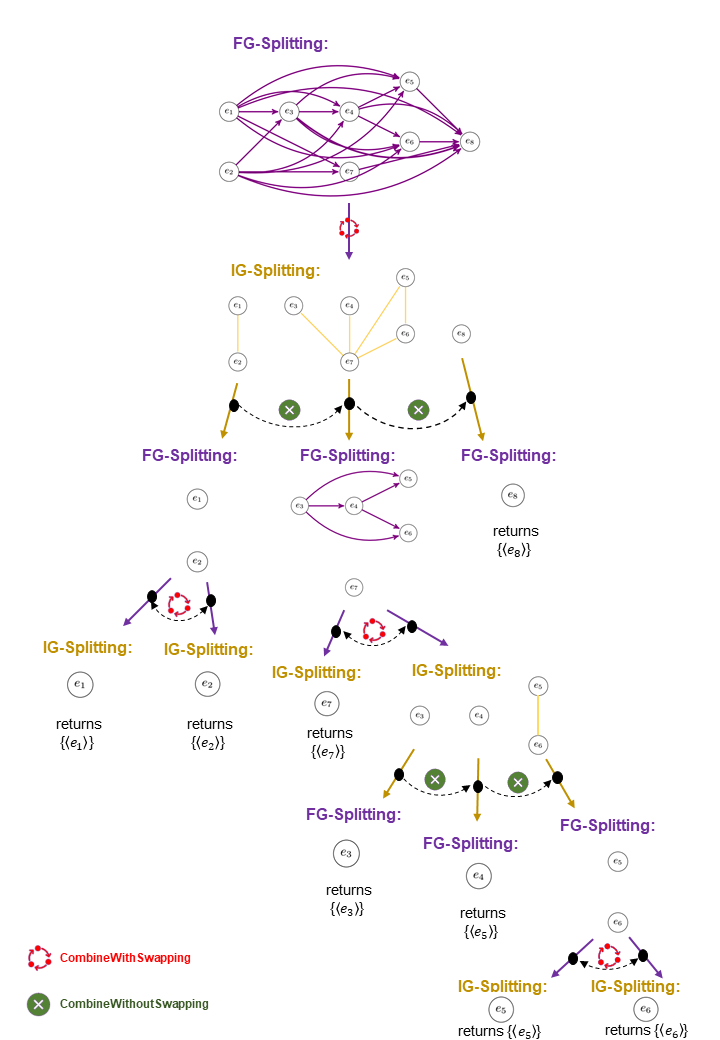
\includegraphics[width=1 \columnwidth]{figures/alg_visualization_paper.png}
	\caption{A visualization of the full recursion tree of the \textsc{ValidPermutations} algorithm when applied on the example event set from Table \ref{table:8 events}.}
	\label{fig: algorithm visualization}
	%width=1\columnwidth
\end{figure}
%
%
%
%
%
%
% 
Figure \ref{fig: algorithm visualization} provides a visualization of all recursion rounds of Algorithm \ref{alg:valid permutations} on input set $E$ from Table \ref{table:8 events}.
The directed graphs with violet arcs represent the subgraphs induced from the follows graph.
The violet arcs pointing outwards from any violet graph each represent a connected component of that graph.
As we explained earlier, the valid sequences of these violet components are then merged together with swapping.
The red circling lines symbolize the \textsc{CombineWithSwapping} method on these components.
The undirected graphs with yellow edges show the subgraphs induced by the interval graph.
Similarly, the yellow arcs pointing outwards from any yellow graph each represent a connected component of that graph.
The valid sequences from these components are merged back together by preserving a fixed ordering.
The green cross in the visualization symbolizes the cartesian product over those components computed by the \textsc{CombineWithoutSwapping} method.
In this example, the recursion breaks as all subgraphs are split up until they consist of single nodes.
The violet and yellow graphs guide the top-down view of the algorithm, starting from the original single follows graph and partitioning the vertex set in each round until we arrive at trivial nodes.
The green cross and the red circle over the arrows connecting different components guide the bottom-up view of the algorithm.
They indicate how valid subsequences are to be merged together in every step, starting from the trivial singleton sequences and ending with the full sequences of size $|E|$.
%
%
%
%
%
%
%Then Algorithm \ref{alg: FollowsGraph Splitting} is called on input $(\mathcal{F}(E),\mathcal{I}(E),E)$.
%$\mathcal{F}(E)$ has only one component, for which Algorithm \ref{alg: IntervalGraph Splitting} is called.
%In lines 4-9, the connected components of the interval graph $\mathcal{I}(E)$ are computed and ordered into $\langle \{e_1,e_2\},\{e_3,e_4,e_5,e_6,e_7\},\{e_8,\} \rangle$.
%Then for each of them, Algorithm \ref{alg: PrecGraph Splitting} is called again with the corresponding vertex subset:\\
%- On component $\{e_1,e_2\}$: $\mathcal{F}[\{e_1,e_2\}]$ has two components, namely the two single nodes.
%When calling Algorithm $\ref{alg: IntervalGraph Splitting}$ on each one of these nodes, the trivial outputs $\{\langle e_1 \rangle\}, \{\langle e_2 \rangle\}$ are yielded.
%In line 9 (Alg. \ref{alg: PrecGraph Splitting}) these two are combined with swapping by Algorithm \ref{alg:combine with} which yields set $\{ \langle e_1, e_2 \rangle, \langle e_2, e_1 \rangle \}$.\\
%- On component $\{e_3,e_4,e_5,e_6,e_7\}$: $\mathcal{F}[\{e_3,...,e_7\}]$ has two connected components, namely $\{e_3,e_4,e_5,e_6\}$ and $\{e_7\}$.
%Algorithm \ref{alg: IntervalGraph Splitting} applied to $\{e_7\}$ yields the trivial set $\{e_7\}$.
%On input $\{e_3,e_4,e_5,e_6\}$, it computed the interval graph and sorts its components into $\langle \{e_3\}, \{e_4\}, \{e_5,e_6\} \rangle$.
%Algorithm \ref{alg: PrecGraph Splitting} applied to the three directed subgraphs induced by these three vertex sets yields (after another round of calling Alg. \ref{alg: IntervalGraph Splitting} and \ref{alg:combine with}) the outputs $\{ \langle e_3 \rangle \}$, $\{ \langle e_4 \rangle \}$ and $\{ \langle e_5,e_6 \rangle, \langle e_6, e_5 \rangle \}$ respectively.
%These three outputs have exactly this order when they are combined without swapping in line 14 of Algorithm \ref{alg: IntervalGraph Splitting}.
%This yields the set $\{ \langle e_3,e_4,e_5,e_6\rangle, \langle e_3,e_4,e_6,e_5 \rangle\}$.
%On a later round, the sets $\{\langle e_3,e_4,e_5,e_6\rangle, \langle e_3,e_4,e_6,e_5 \rangle\}$ and $\{\langle e_7 \rangle\}$ are combined with swapping: In this case, event $e_7$ is put to every possible position of each of the longer lists (\textcolor{red}{lines 10-16}) of Algorithm \ref{alg:combine with} yielding 10 valid permutations.\\
%- On component $\{e_8\}$: Algorithm \ref{alg: IntervalGraph Splitting} yields the trivial set $\{\langle e_8 \rangle\}$.

%In the end, the sets yieled for components $\{e_1,e_2\}$, $\{e_3,e_4,e_5,e_6,e_7\}$ and $\{e_8\}$ are all combined in this order into full sequences of length 8 in line 14 of Algorithm \ref{alg: IntervalGraph Splitting}, yielding in the end the set of all $20 ~ (2 \times 10 \times 1)$ topological sortings of the original $\mathcal{F}(E)$ and this way $\mathcal{R}_e(E)$ conatining:
Applied on the example event set, the \textsc{ValidPermutations} algorithm yields the following 20 sequences:
\begin{itemize}
\item $\langle e_1,e_2,e_3,e_4,e_5,e_6,e_7,e_8\rangle$ 
\item $\langle e_1,e_2,e_3,e_4,e_6,e_5,e_7,e_8\rangle$ 
\item $\langle e_1,e_2,e_3,e_4,e_5,e_7,e_6,e_8\rangle$
\item $\langle e_1,e_2,e_3,e_4,e_6,e_7,e_5,e_8\rangle$ 
\item $\langle e_1,e_2,e_3,e_4,e_7,e_5,e_6,e_8\rangle$
\item $\langle e_1,e_2,e_3,e_4,e_7,e_6,e_5,e_8\rangle$
\item $\langle e_1,e_2,e_3,e_7,e_4,e_5,e_6,e_8\rangle$
\item $\langle e_1,e_2,e_3,e_7,e_4,e_6,e_5,e_8\rangle$
\item $\langle e_1,e_2,e_7,e_3,e_4,e_5,e_6,e_8\rangle$
\item $\langle e_1,e_2,e_7,e_3,e_4,e_6,e_5,e_8\rangle$
\item $\langle e_2,e_1,e_3,e_4,e_5,e_6,e_7,e_8\rangle$ 
\item $\langle e_2,e_1,e_3,e_4,e_6,e_5,e_7,e_8\rangle$ 
\item $\langle e_2,e_1,e_3,e_4,e_5,e_7,e_6,e_8\rangle$
\item $\langle e_2,e_1,e_3,e_4,e_6,e_7,e_5,e_8\rangle$ 
\item $\langle e_2,e_1,e_3,e_4,e_7,e_5,e_6,e_8\rangle$
\item $\langle e_2,e_1,e_3,e_4,e_7,e_6,e_5,e_8\rangle$
\item $\langle e_2,e_1,e_3,e_7,e_4,e_5,e_6,e_8\rangle$
\item $\langle e_2,e_1,e_3,e_7,e_4,e_6,e_5,e_8\rangle$
\item $\langle e_2,e_1,e_7,e_3,e_4,e_5,e_6,e_8\rangle$
\item $\langle e_2,e_1,e_7,e_3,e_4,e_6,e_5,e_8\rangle$
\end{itemize}
%
%
%
%
%
%
%
\section{Complexiy Analysis}
The \textsc{ValidPermutations} Algorithm (\ref{alg:valid permutations}) computes the set of correct evaluation orders on the input event set by using the interval graph trick, that is, partitioning the event set into subsets that can be ordered in time and then recursively computing the valid orderings for the smaller event sets.
When computing the interval graph on some given event set manages to partition it further, then the subsets for which the orderings have to be computed get smaller and smaller.
The recursion breaks on trivial components of size one yielding the trivial singleton sequence.
If the interval graph trick does not do the trick, that is, the input event set cannot be divided into smaller timely comparable event subsets, then the method relies on the naive \textsc{TopologicalSortings} algorithm (\ref{alg:topo sortings}) to compute the correct evaluation orders on the current event set.
In both scenarios, the recursion breaks at some point and the smaller sequences are merged back together until they yield the full valid sequences.
Thus the \textsc{ValidPermutations} algorithm always terminates.

It is easy to determine that for the naive method, that is, constructing the follows graph (Algorithm \ref{alg:follows graph}) and then applying the \textsc{TopologicalSortings} method (\ref{alg:topo sortings}) on it, the runtime is asymptotic.
Constructing the follows graph in Algorithm \ref{alg:follows graph} requires $\mathcal{O}(n^2)$.
The \textsc{TopologicalSortings} algorithm goes through all possible permutations over the vertex set of the input graph which runs in $\mathcal{O}(n!)$.
Then it checks validity for every single one of them, which costs $\mathcal{O}(n)$ for going through each vertex and $\mathcal{O}(n)$ to check whether the current vertex is in the \textit{previous} set, resulting in $\mathcal{O}(n^2)$ for each permutation.
Thus the total running time of the naive method is $\mathcal{O}(n^2) + \mathcal{O}(n^2 \cdot n!) = \mathcal{O}(n!)$.

Determining the complexity of the \textsc{ValidPermutations} algorithm is not as straighforward, since the runtime heavily depends on the graph structure of the follows graph and whether the algorithm falls back into the naive method or not.
The graph structure affects how well the interval graph trick works on the input event set and how many recursion rounds are completed before termination.
First, we analyze the runtime assuming that the recursion only breaks on trivial components, that is, the naive method is never called.
The visualization of the example run in Figure \ref{fig: algorithm visualization} can be helpful when conducting this runtime analysis.
A full recursion round consists of calling \textsc{FollowsGraphSplitting} and \textsc{IntervalGraphSplitting} once.
In the visualization, this would consist of a round of a violet and yellow graphs pair.
Computing the initial follows- and interval graph in Algorithm \ref{alg:valid permutations} each costs $\mathcal{O}(n^2)$ resulting in $\mathcal{O}(2n^2)$.
In each recusion round a follows graph and an interval graph are computed, which runs in $\mathcal{O}(2n^2)$, and for each graph the connected components are detected, which results in an additional $\mathcal{O}(2n^2)$.
Sorting the components in the \textsc{IntervalGraphSplitting} method runs in $\mathcal{O}(n \cdot log(n))$.
In total, these operations contribute to a runtime of $ \mathcal{O}(2n^2)+\mathcal{O}(2n^2)+\mathcal{O}(n \cdot log(n)) = \mathcal{O}(n^2)$ for each round.
Suppose $S$ is the set of all valid permutations over the input event set.
Since every $s \in S$ is reconstructed from its subsequences by explicitly dictating only the valid positions for each element from the event set, each valid sequence from $S$ contributes $\mathcal{O}(1)$ in each recusion round.
In total this is $\mathcal{O}(|S|)$.
If $d$ is the maximal recursion depth, then the total runtime is $d \cdot \big(\mathcal{O}(n^2) + \mathcal{O}(|S|) \big) = \mathcal{O}(dn^2 + d|S|)$.
On the other hand, if the recursion breaks by returning to the naive method because that particular subset of the input event set can not be further fragmentized, then there is an added runtime which is asymptotic in the size of that component.
That is why for the general case, the runtime method is $\mathcal{O}(dn^2 + d|S| + k!)$ where $k$ is the size of the biggest component whose valid sequences are determined through the naive method.
The impact of the fallback into the naive method may however be not as dramatic if $k$ is a lot smaller than $n$.
Note that regardless of whether the naive method is called at some point, in the worst-case scenario, the runtime is still asymptotic.
If a very high number (close to $n!$) of sequences are valid, then all those sequences will have to be constructed, therefore the $|S|$ term is also very large. 

Next we show two input examples, one on which the \textsc{ValidPermutations} algorithm performs particularly well compared to the naive method, and one on which its execution is very similar to the naive method. 
%
%
%
%
\begin{figure}[h!]
\centering

	\begin{tikzpicture}[->,>=stealth',shorten >=1pt,node 						distance=2.5cm,auto,main node/.style={circle,draw,align=center}]
	%\draw [help lines] (0,0) grid (7,3);
	\node[main node, label=above: ${[0,2]}$] (A) at (1,1) {$e_1$};
	\node[main node, label=above: ${3}$] (B) at (3,1) {$e_2$};
	\node[main node, label=above: ${[5,6]}$] (C) at (5,1) {$e_3$};
	\node[main node, label=above: ${[8,10]}$] (D) at (7,1) {$e_4$};
	\node[main node, label=above: ${11}$] (E) at (9,1) {$e_5$};
	
	\path
	(A) edge (B)
	(A) edge [bend right] (C)
	(A) edge [bend right] (D)
	(A) edge [bend right] (E)
	(B) edge (C)
	(B) edge [bend right] (D)
	(B) edge [bend right] (E)
	(C) edge (D)
	(C) edge [bend right] (E)
	(D) edge (E)

	;
	\end{tikzpicture}
	
	\vspace{1cm}
	
	\begin{tikzpicture}[->,>=stealth',shorten >=1pt,node 						distance=2.5cm,auto,main node/.style={circle,draw,align=center}]
	%\draw [help lines] (0,0) grid (7,3);
	\node[main node, label=above: ${[0,2]}$] (A) at (1,1) {$e_1$};
	\node[main node, label=above: ${3}$] (B) at (3,1) {$e_2$};
	\node[main node, label=above: ${[5,6]}$] (C) at (5,1) {$e_3$};
	\node[main node, label=above: ${[8,10]}$] (D) at (7,1) {$e_4$};
	\node[main node, label=above: ${11}$] (E) at (9,1) {$e_5$};
	
	\path


	;
	\end{tikzpicture}
	\caption{The upper graph shows the follows graph of some uncertain process instance where despite uncertainty in timestamps, no events have overlapping time intervals.
	The lower graph is the corresponding interval graph.}
	\label{fig: runtime example 1}
\end{figure}
%
%
%
%
%
\begin{figure}[h!]
\centering

	\begin{tikzpicture}[->,>=stealth',shorten >=1pt,node 						distance=2.5cm,auto,main node/.style={circle,draw,align=center}]
	%\draw [help lines] (0,0) grid (10,5);
	\node[main node] (A) at (0,1) {$e_1$};
	\node[main node] (B) at (0,4) {$e_2$};
	\node[main node] (C) at (3,1) {$e_5$};
	\node[main node] (D) at (3,2.5) {$e_4$};
	\node[main node] (E) at (3,4) {$e_3$};
	
	\path
	(A) edge (C)
	(B) edge (C)
	(B) edge (D)
	(B) edge (E)

	;
	%\end{tikzpicture}
	%
	%
	%
	%
	%\begin{tikzpicture}[-,>=stealth',shorten >=1pt,node 						distance=2.5cm,auto,main node/.style={circle,draw,align=center}]
	\node[main node] (A) at (6,1) {$e_1$};
	\node[main node] (B) at (6,4) {$e_2$};
	\node[main node] (C) at (9,1) {$e_5$};
	\node[main node] (D) at (9,2.5) {$e_4$};
	\node[main node] (E) at (9,4) {$e_3$};
	
	\path
	(A) edge [-] (B)
	(A) edge [-] (D)
	(A) edge [-] (E)
	(C) edge [-] (D)
	(C) edge[bend right,-] (E)
	(D) edge [-] (E)
	;
	\end{tikzpicture}
	\caption{The left graph shows the follows graph of some uncertain process instance and the right graph shows its corresponding interval graph.}
	\label{fig: runtime example 2}
\end{figure}
%
%
%
%
Consider an event set of 5 events whose follows -and interval graph are shown in Figure \ref{fig: runtime example 1}.
Note that the corresponding behavior graph of this event set would be a path, indicating that there is only one valid permutation.
When applied on this example, the \textsc{ValidPermutations} algorithm constructs the graphs from Figure \ref{fig: runtime example 1} and already during the first recursion round the  \textsc{IntervalGraphSplitting} method detects the 5 trivial components and orders them.
The unique valid sequence is obtained as a cartesian product from the 5 sets containing the singleton sequences.
In the naive method, the set of topological sortings are computed on the follows graph.
Since there are 5 events, all 5!=120 permutations are considered and checked for validity, even though only one is a topological sorting and thus a correct evaluation order.

Now consider the 5 events in the example from Figure \ref{fig: runtime example 2} which shows their corresponding follows- and interval graph.
After computing both graphs, already in the first recursion round of \textsc{ValidPermutations} the \textsc{IntervalGraphSplitting} method detects that the interval graph has only one connected component.
This indicates that the event set can not be partitioned into comparable subsets.
At this point the set of topological sortings is computed using the naive \textsc{TopologicalSortings} method, which goes through all 5!=120 possible permutations, even though                                only 18 of them are correct.   
%
%
%
%
%
%
%\newpage
\section{Runtime Experiments}
Both the naive method (Algorithm \ref{alg:topo sortings}) and the novel way (Algorithm \ref{alg:valid permutations}) of obtaining the correct evaluation orders over a set of uncertain events are implemented in Python \textcolor{red}{add github in footnote}.
In this subsection we show the results of two series of experiments that aim to compare the running times of the new \textsc{ValidPermutations} algorithm and the naive \textsc{TopologicalSortings} method.
In both of them, the input is a set of events represented as triples containing the event ID, the minimum and maximum timestamp.
Each event set is generated the following way: First we generate a synthetic log containing a single certain trace of a specific length using the PM4Py framework \cite{pm4py}.
More specifically, given a parameter $n$, we first generate a petri net with $n$ visible transitions which can only replay a single sequence.
Then we run a simulator on this petri net to obtain synthetic event data in form of a log containing the unique replayable trace.
To add uncertainty to the data, we use the functionalities provided by the PROVED \cite{proved} library.
More specifically, we make use of a function that given a certain trace and a parameter $p$, randomly generates minimum and maximum timestamp values for the events so that the probability that any two subsequent events overlap is $p$.
Timestamps are represented by their distance from the \textit{Unix Epoch}.
We let both algorithms run on identical events sets and measure the elapsed time for each of them.
The plotted performance results are obtained as an average of 10 runs of the corresponding experiment.

In the first series of experiments, we compare the novel algorithm \textsc{ValidPermutations} with the naive \textsc{TopologicalSortings} method by using an input event set of a fixed length $n=8$ where the timestamp uncertainty is generated with increasing probability $p$.
%
%
%
\begin{figure}
	\centering
	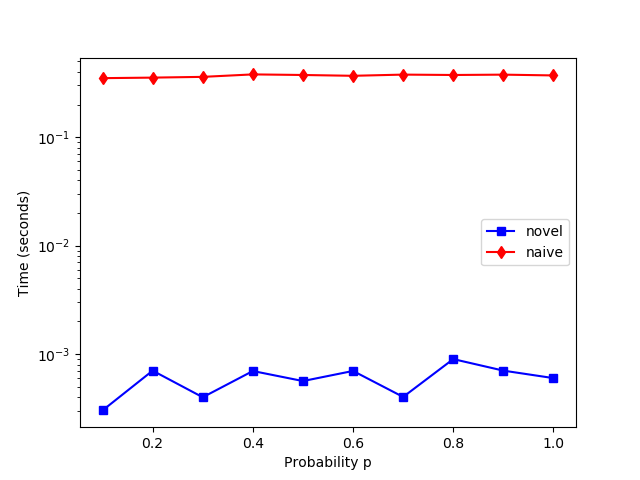
\includegraphics[width=0.8\columnwidth]{figures/n_fixed_8_logscale.png}
	\caption{Time in seconds for computing the correct evaluation orders on a set of 8 events with timestamp uncertainty.}
	\label{fig: series1}
	%width=1\columnwidth
\end{figure}
%
%
%

As expected, the results in Figure \ref{fig: series1} show that the \textsc{ValidPermutations} Algorithm terminates in a fraction of the time required by the naive method of the \textsc{TopologicalSortings} algorithm.
As we explained before, the new algorithm performs particularly well if the input event set can be partitioned into comparable subsets.
This avoids the asymptotic runtime of checking many invalid permutations.
In the second series of experiments, the parameter $p$ for generating timestamp uncertainty is kept fixed at either $0.2$ or $0.8$, while the size $n$ of the input event set varies from 1 to 10.
%To generate such event sets with rather few overlappings, we use a probability $p=0.4$ when adding uncertain timestamps to the data and compare the runtime for different input sizes.
%
%
%
\begin{figure}
	\centering
	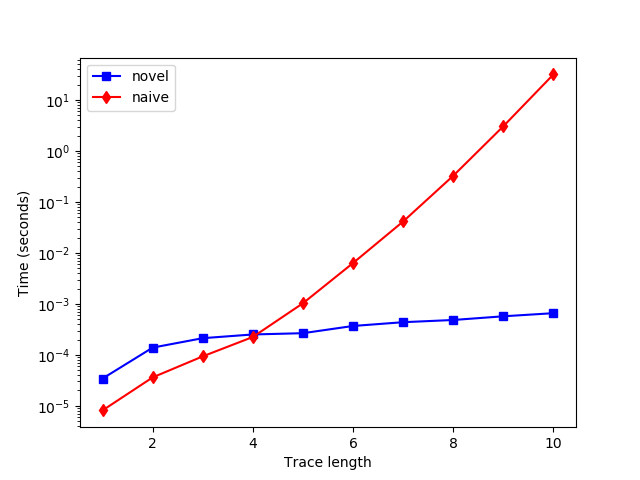
\includegraphics[width=0.8\columnwidth]{figures/fixed_p_08_logscale.png}
	\caption{Time in seconds for computing the correct evaluation orders on an event set of increasing size. The probability of two neighboring events to have overlapping timestamps is $p=0.8$.}
	\label{fig: series21}
	%width=1\columnwidth
\end{figure}
%
%2
%
As expected, Figures \ref{fig: series21} and \ref{fig: series22} show how the benefit of fragmentizing the input event set to avoid checking all permutations increases dramatically for increasing input size $n$.
%
%
%
\begin{figure}
	\centering
	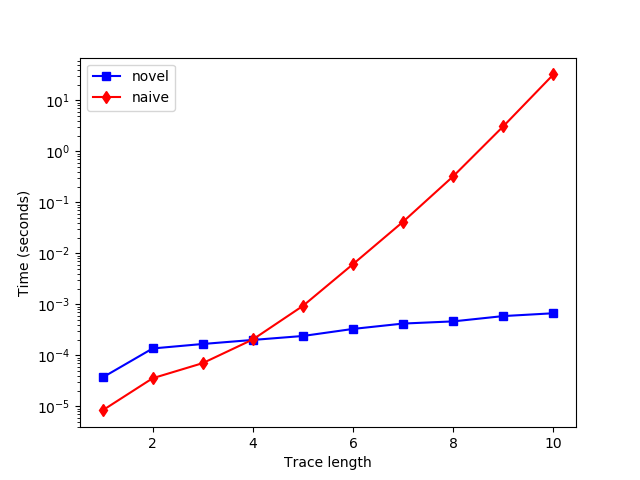
\includegraphics[width=0.8\columnwidth]{figures/fixed_p_02_logscale.png}
	\caption{Time in seconds for computing the correct evaluation orders on an event set of increasing size. The probability of two neighboring events to have overlapping timestamps is $p=0.2$.}
	\label{fig: series22}
	%width=1\columnwidth
\end{figure}
%
%
%
%
%
%
%
%
In summary, our experiments show that the novel algorithm has a much better performance than the naive method and the runtimes between the two differ increasingly with increasing input size.
This might lie on the fact that the function we use to add timestamp uncertainty to the certain data mostly creates timestamp overlappings of neighboring events.
Such uncertain event sets offer a well partitionable input to the novel method making it less affectable by the input size, while the runtime of the naive algorithm still increases asymptotically.
While the novel algorithm still might show a runtime in seconds that is noticeably above 0 for larger inputs, the naive method is far too slow on those inputs for its runtime to be plotted meaningfully.
%
%
%
%
%
%\newpage
\section{Event Trace Realizations with Indeterminate Events}
In the previous section we saw how we can compute a set of valid permutations for any event set $E$.
Note that in the computed valid permutations, every event of $E$ appears in all permutations yielded by the algorithm.
Thus the computed valid permutations cover all correct evaluation orders on $(E, \prec_{\mathcal{E}})$ if and only if all events in $E$ are determinate.
Otherwise, we have to extend the set of valid permutations by the missing sequences in which indeterminate events do not appear.
This can be done the following way:
Let $E$ be an event set and let $\overline{E}=\{e \in E \mid \pi_o(e) \neq  ~! \vee \pi_o(e)=f_O \in F_{\mathcal{U}_O} \wedge f_O(?) > 0 \}$ denote the set of indeterminate events from $E$.
Similarly, we can indicate indeterminate events by overlining them. 
This way, for every valid permutation $s$ we have computed in Algorithm \ref{alg:valid permutations}, we add the remaining $2^{|\overline{E}|} - 1 $ sequences missing from the event trace realizations. \\ 
%
For example, let
$E=\{e_1,\overline{e_2},\overline{e_3},e_4\}$ be some event set and suppose 
$\{ \langle e_1,e_2,e_3,e_4 \rangle, \\ 
\langle e_1,e_3,e_2,e_4 \rangle \}$
are the valid permutations computed from Algorithm \ref{alg:valid permutations}.
The missing sequences are $\langle e_1, e_2, e_4 \rangle, \langle e_1, e_3, e_4 \rangle$ and $\langle e_1, e_4 \rangle$.
Finally, we update $\mathcal{R}_e(E)$ so that it contains all 5 possible event trace realizations.

From now on we assume that the computed set $\mathcal{R}_e(E)$ for some event set $E$ already contains all event trace realizations of $E$.
%Besides already having a possibly non-empty set $\overline{E} \subseteq E$ containing the indeterminate events, one can also notice whether the case corresponding to $E$ has indeterminate events by looking at the lengths of the sequences of event trace realizations.
%These sequences have all length $|E|$ when there are no indeterminate events.
%
%
%
%
%
%
%
